{
\newcommand{\raised}[3]{\fill[white] #1;\fill[white] #2;\fill[white] #3;\draw #1;\draw #2;\draw #3;}

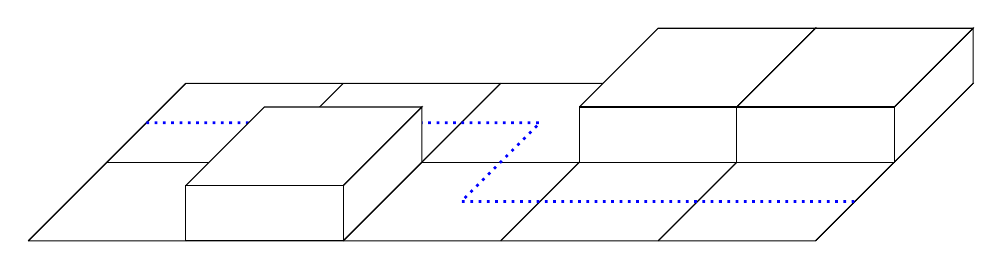
\begin{tikzpicture}[scale=2]
\def\rlvl{0.35}

% Grid
\draw (0,0) -- (1,1) -- (6,1) -- (5,0) -- (0,0);
\foreach \x in {0,1,...,5} {
    \draw (\x,0) -- (\x+1,1);
}
\draw (0.5,0.5) -- (5.5,0.5);

%Path
\draw[line width=0.35mm, blue, dotted] (0.75,0.75) -- (0.75+2.5,0.75) -- (0.75+2.5-0.5,0.75-0.5) -- (0.75+2.5-0.5+2.5,0.75-0.5);

% Raised squares
\raised{(1,0) rectangle (2,\rlvl)}{(2,0) -- (2.5,0.5) -- (2.5,0.5+\rlvl) -- (2,\rlvl)}{(2,\rlvl) -- (2.5,0.5+\rlvl) -- (1.5,0.5+\rlvl) -- (1,\rlvl)}
\raised{(1+2.5,0+0.5) rectangle (2+2.5,\rlvl+0.5)}{(2+2.5,0+0.5) -- (2.5+2.5,0.5+0.5) -- (2.5+2.5,0.5+\rlvl+0.5) -- (2+2.5,\rlvl+0.5)}{(2+2.5,\rlvl+0.5) -- (2.5+2.5,0.5+\rlvl+0.5) -- (1.5+2.5,0.5+\rlvl+0.5) -- (1+2.5,\rlvl+0.5)}
\raised{(1+2.5+1,0+0.5) rectangle (2+2.5+1,\rlvl+0.5)}{(2+2.5+1,0+0.5) -- (2.5+2.5+1,0.5+0.5) -- (2.5+2.5+1,0.5+\rlvl+0.5) -- (2+2.5+1,\rlvl+0.5)}{(2+2.5+1,\rlvl+0.5) -- (2.5+2.5+1,0.5+\rlvl+0.5) -- (1.5+2.5+1,0.5+\rlvl+0.5) -- (1+2.5+1,\rlvl+0.5)}
\end{tikzpicture}
}